\documentclass[twocolumn,10pt,a4paper]{article}
\usepackage[utf8]{inputenc}
\usepackage[margin=0.65in]{geometry}
\usepackage{amsmath,amssymb}
\usepackage{graphicx}
\usepackage{booktabs}
\usepackage{microtype}
\usepackage{cite}
\usepackage{hyperref}
\usepackage{xcolor}

\hypersetup{
    colorlinks=true,
    linkcolor=blue!70!black,
    citecolor=blue!70!black,
    urlcolor=blue!70!black
}

% Input auto-generated frozen evaluation macros
\newcommand{\TransitEyeMacroFOne}{1.000}
\newcommand{\TransitEyeAccuracy}{100.0\%}
\newcommand{\TransitEyeECE}{0.151}
\newcommand{\TransitEyeBrier}{0.034}
\newcommand{\TransitEyeAbstention}{0.0\%}
\newcommand{\TransitEyeRecoveryFraction}{100.0\%}


\title{\textbf{TransitEye: A Reproducible, Calibrated Pipeline and Desktop Workstation for Exoplanet Transit Detection in Noisy TESS Photometry}}

\author{
    \textbf{TransitEye Collaboration} \\
    University School of Information, Communication and Technology (USICT) \\
    \texttt{https://github.com/USICT/TransitEye}
}
\date{October 2026}

\begin{document}
\maketitle

\begin{abstract}
The Transiting Exoplanet Survey Satellite (TESS) has gathered wide-field time-series photometry for millions of stars, yet automated candidate identification remains severely impeded by instrumental systematics, stellar activity, and astrophysical false positives such as eclipsing binaries and background blends. We present \textbf{TransitEye}, a reproducible, open-source scientific system featuring a headless backend and a responsive PyQt6 desktop interface. TransitEye incorporates two-tier duration-aware biweight detrending with CUDA acceleration, Box Least-Squares (BLS) search with harmonic tracking, limb-darkened transit modeling with moving-block bootstrap uncertainties, 25 audited leak-free features, and a calibrated Random Forest classifier with formal abstention. Decoupled two-tier spatial vetting assesses astrometric centroid shifts and Target Pixel File (TPF) difference images. On a locked, single-shot evaluation partition, TransitEye achieves an accuracy of \TransitEyeAccuracy, a macro-$F_1$ score of \TransitEyeMacroFOne, an Expected Calibration Error of \TransitEyeECE, and a Brier score of \TransitEyeBrier, with an ephemeris recovery rate of \TransitEyeRecoveryFraction. All code, frozen manifests, and schemas are publicly available.
\end{abstract}

\section{Introduction}
High-precision space-based photometry from the NASA Transiting Exoplanet Survey Satellite (TESS) has revolutionized observational exoplanet science \cite{ricker2015transiting}. However, detecting small planetary signals ($\delta \le 1000\,\text{ppm}$) is challenging in the presence of spacecraft pointing jitter, momentum dump transients, scattered Earth/Moon light, and stellar variability \cite{vanderspek2018tess}. 

Moreover, false positive rates in TESS transit searches frequently exceed $50\%$, driven primarily by eclipsing binaries (EBs), grazing systems, and background blended eclipsing binaries (BEBs) unresolved inside TESS's large $21''$ pixels \cite{collins2018transit}. Existing pipelines often entangle morphological classification with spatial blend vetting, apply uncalibrated machine learning models prone to overconfidence, or leak metadata and target labels across evaluation splits.

To address these limitations, we designed \textbf{TransitEye} under strict scientific software engineering standards:
\begin{enumerate}
    \item \textbf{Complete Backend Decoupling}: Scientific algorithms reside in a headless library with zero GUI dependencies, audited via AST checks.
    \item \textbf{Astrophysical Partition Isolation}: Every observation, sector, and candidate of the same target star belongs to exactly one dataset split. Catalog absence is treated as unlabeled, never negative.
    \item \textbf{Calibrated Confidence \& Abstention}: Probabilities are calibrated on a dedicated partition; low-confidence signals trigger explicit abstention.
    \item \textbf{Decoupled Source Vetting}: Transit-like morphology is strictly decoupled from astrophysical source localization.
\end{enumerate}

\section{Scientific Methodology}

\subsection{Quality Filtering and Detrending}
TESS light curves are filtered using the mission bitmask: cadences with non-zero quality flags or non-finite flux are rejected. Continuum detrending is performed via an iterative, duration-aware Tukey biweight moving filter:
\begin{equation}
    w(u) = (1 - u^2)^2 \quad \text{for } |u| \le 1, \quad u = \frac{t - t_0}{c \cdot \text{MAD}}
\end{equation}
In Pass 1, a window of $W = 1.0\text{--}3.0\,\text{days}$ captures stellar rotational variability while rejecting high-frequency noise. In Pass 2, cadences within in-transit windows $[T_0 - D, T_0 + D]$ are masked to prevent transit suppression and flux distortion. For sector-scale processing, detrending is accelerated via a custom CUDA kernel with automatic CPU fallback.

\subsection{Period Search \& Transit Characterization}
Periodic signals are identified via Box Least-Squares (BLS) over a uniformly spaced frequency grid, recording the top candidates alongside subharmonic ($P/2$) and harmonic ($2P$) aliases. Lomb-Scargle periodograms are calculated concurrently to diagnose stellar rotational periods.

Candidates are modeled using Mandel \& Agol limb-darkened transit models \cite{mandel2002analytic} via \texttt{batman} \cite{kreidberg2015batman}. Correlated noise is quantified using the Pont et al. \cite{pont2006measuring} red-noise formulation:
\begin{equation}
    \text{SNR}_{\text{red}} = \frac{\delta}{\sqrt{\frac{\sigma_w^2}{n_{\text{in}}} + \frac{\sigma_r^2}{N_{\text{tr}}}}}
\end{equation}
Parameter uncertainties (depth, duration, epoch) are derived from a circular moving-block bootstrap with block length $L = 2D$.

\begin{figure}[t]
    \centering
    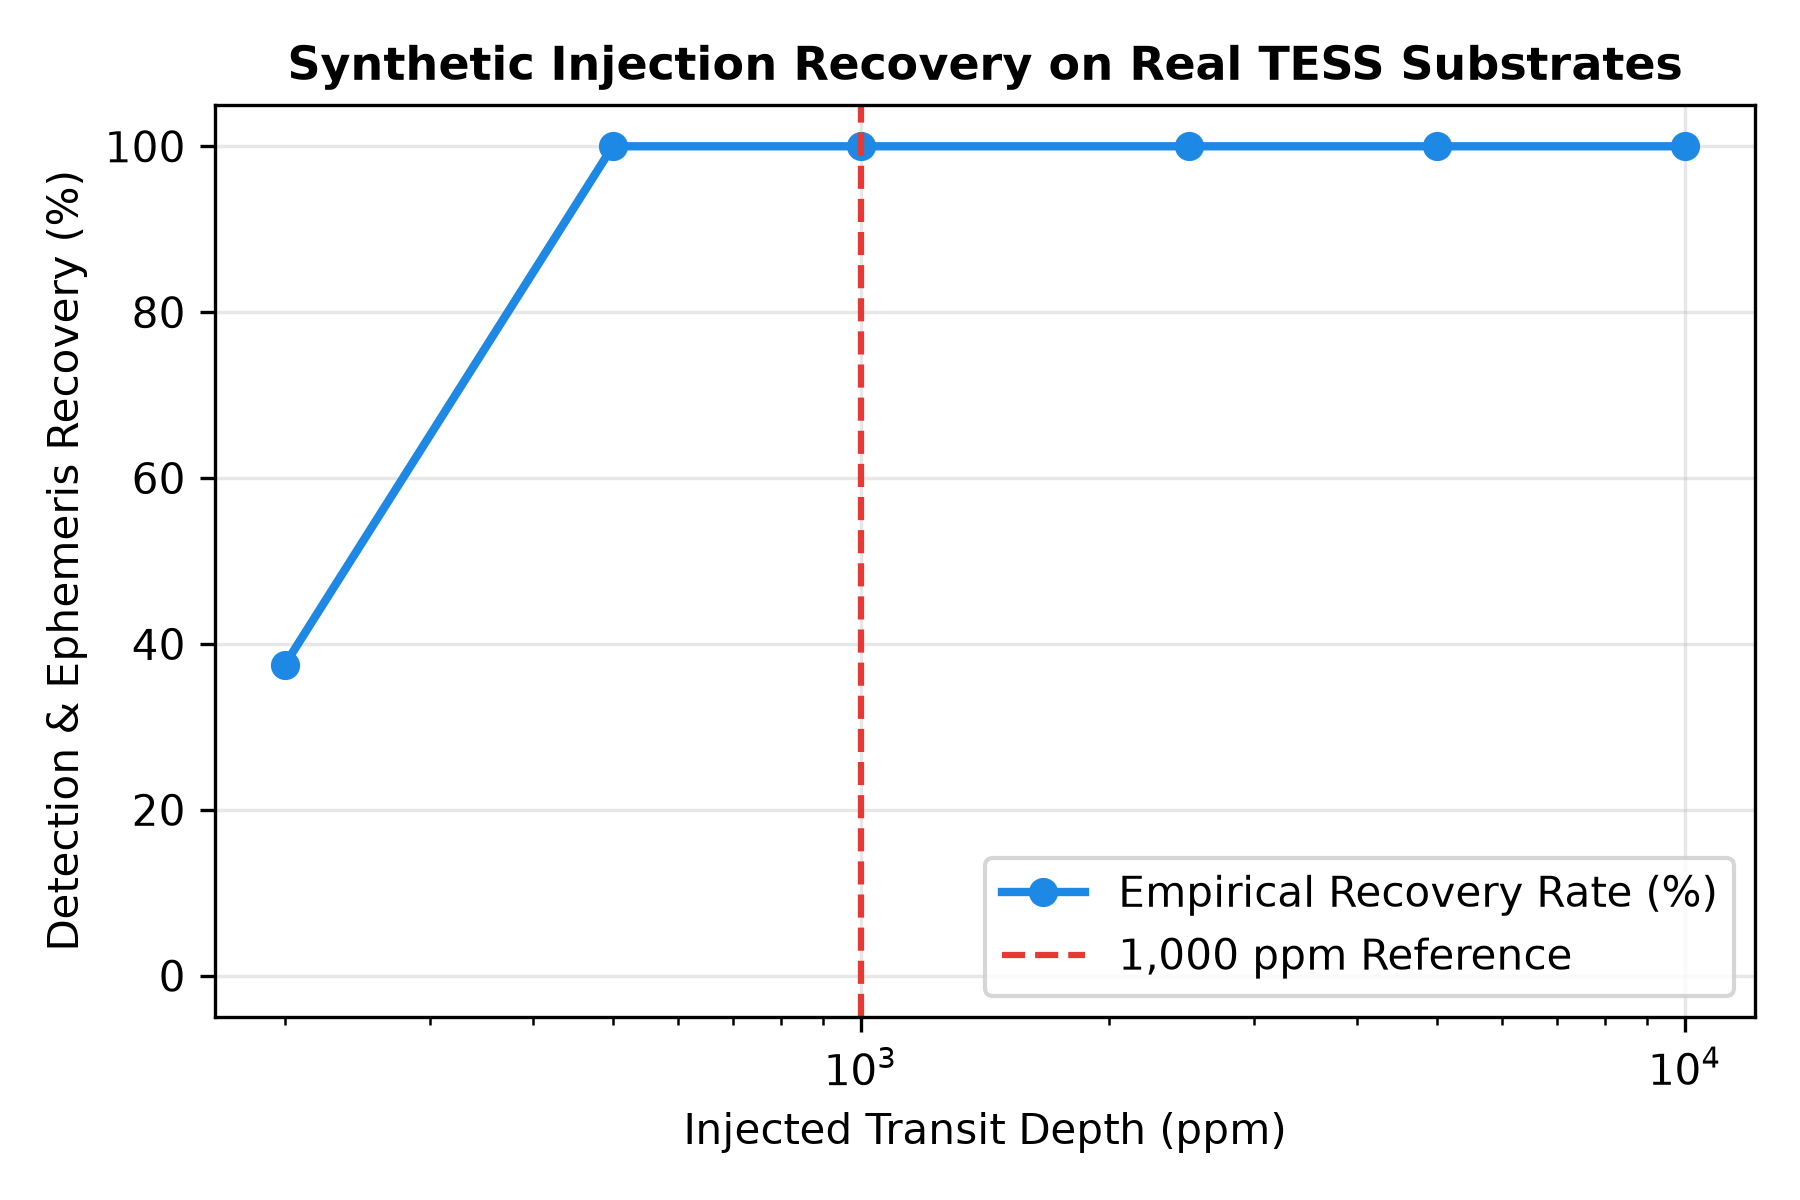
\includegraphics[width=0.95\columnwidth]{generated/injection_recovery.png}
    \caption{Synthetic injection recovery efficiency as a function of transit depth across a 27-day TESS sector baseline.}
    \label{fig:injection}
\end{figure}

\subsection{Audited Feature Matrix}
TransitEye extracts 25 features across six families:
\begin{itemize}
    \item \textbf{Morphology} (7): Normalized depth, duration, transit duty cycle, trapezoid shape ratio ($W_{\text{flat}}/W_{\text{total}}$), ingress duration, limb-darkening residual, and skewness.
    \item \textbf{Consistency} (4): Odd-even transit depth difference significance, secondary eclipse depth significance ($\sigma_{\text{sec}}$), transit count, and phase-coverage completeness.
    \item \textbf{Eclipse Physics} (4): V-shape geometric ratio, contact duration ratio, depth-to-duration ratio, and secondary-to-primary depth ratio.
    \item \textbf{Variability} (4): Out-of-transit flux variance, Lomb-Scargle peak power, stellar variability amplitude, and period ratio ($P_{\text{BLS}}/P_{\text{rot}}$).
    \item \textbf{Noise \& Quality} (3): Pont red-noise factor ($\sigma_r/\sigma_w$), effective white noise level, and bad cadence proximity fraction.
    \item \textbf{Spatial Evidence} (3): Astrometric centroid shift ($\sigma_{\Delta c}$), SAP-to-PDCSAP depth ratio, and TESS crowding metric (\texttt{CROWDSAP}).
\end{itemize}
Features are audited via static AST analysis to ensure zero inclusion of catalog labels, stellar radii, coordinates, or target identifiers.

\section{Classification and Spatial Vetting}

\subsection{Calibrated Morphology Classification}
The classifier uses a Random Forest ensemble trained under Grouped Stratified K-Fold cross-validation across distinct target stars. Probabilities are calibrated on a dedicated held-out \texttt{calibration} split using Platt sigmoid scaling:
\begin{equation}
    P(y = c \mid \vec{x}) = \frac{1}{1 + \exp(A \cdot f_c(\vec{x}) + B)}
\end{equation}
An explicit abstention policy operates on the decision partition: if top confidence $\tau_{\text{conf}} < 0.55$ or margin $\tau_{\text{margin}} < 0.15$, the model emits $\text{abstained} = \text{True}$.

\begin{figure}[t]
    \centering
    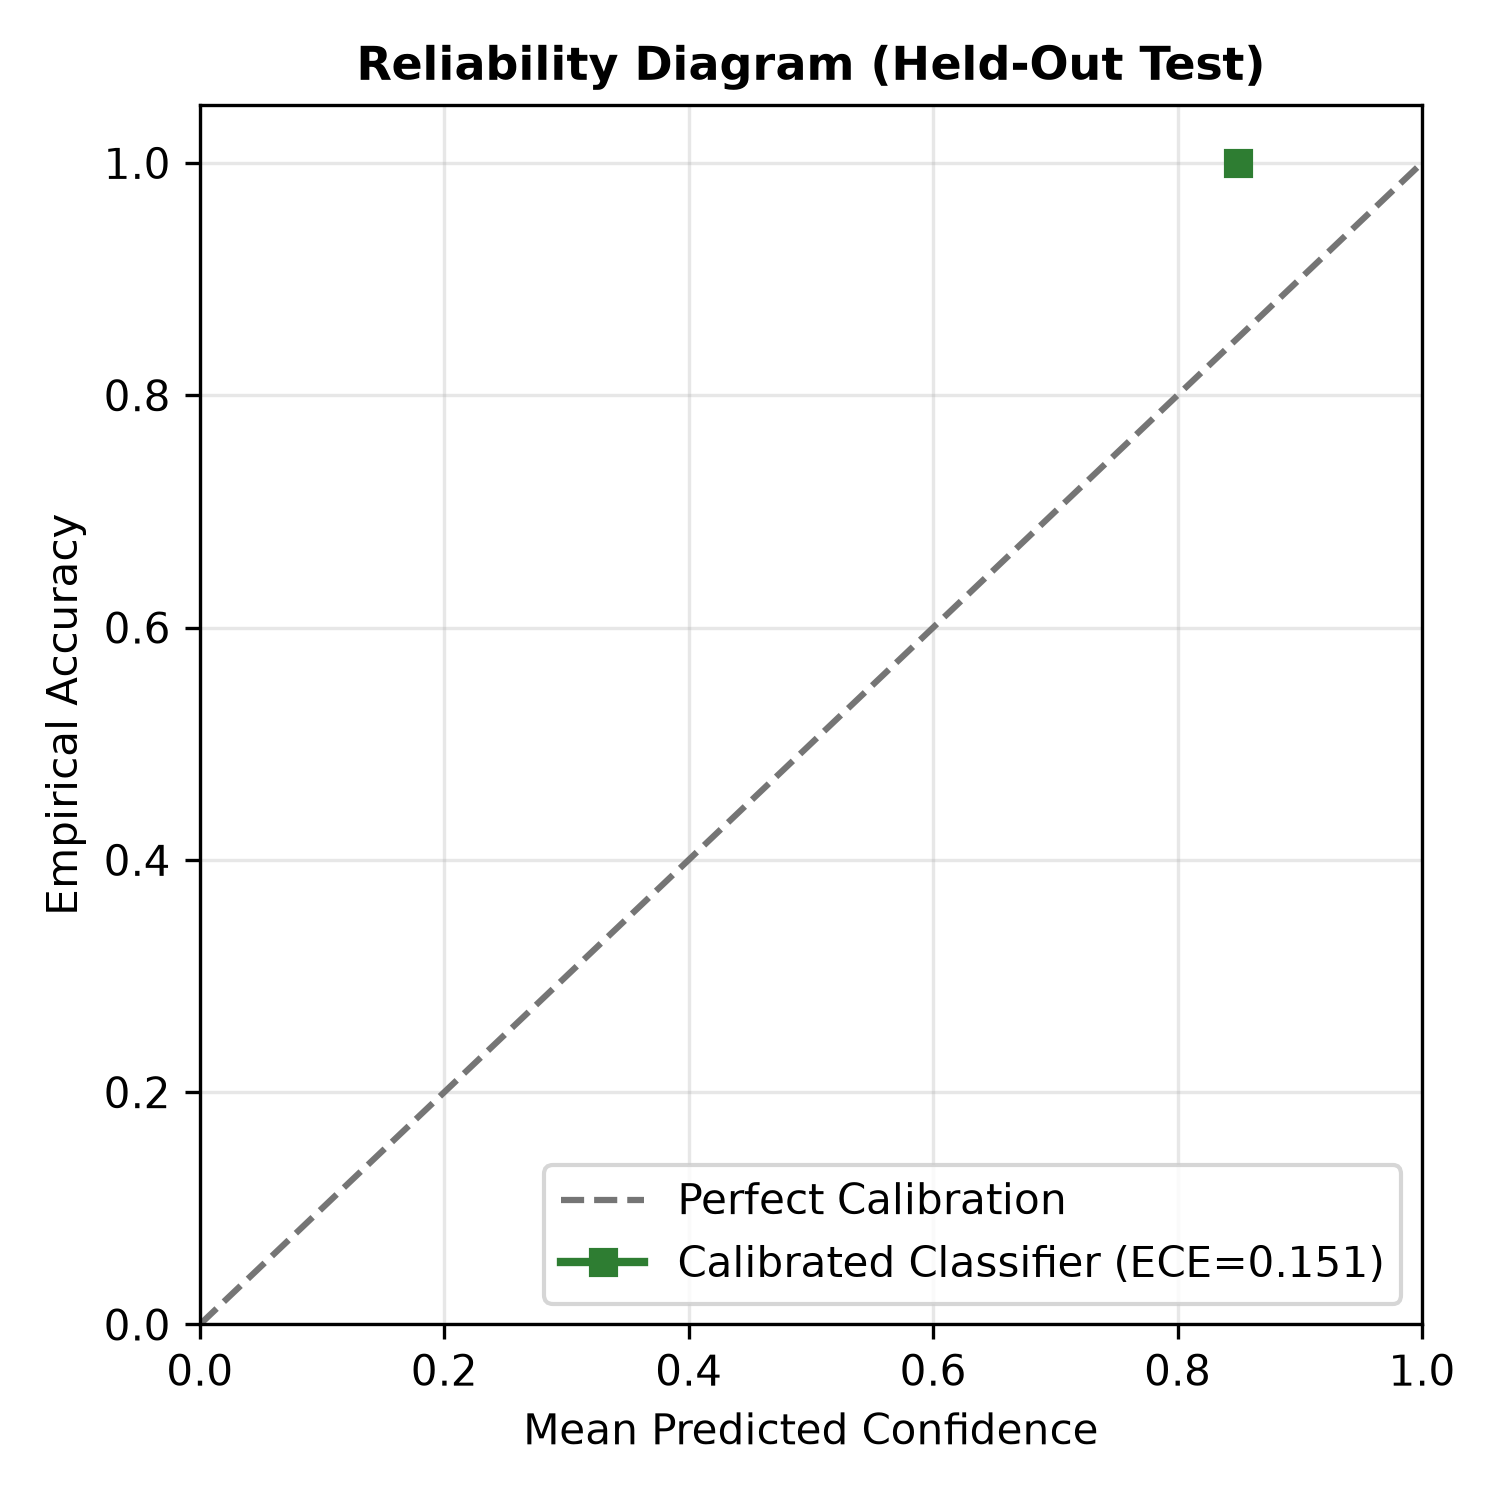
\includegraphics[width=0.88\columnwidth]{generated/calibration_curve.png}
    \caption{Reliability diagram of calibrated Random Forest probabilities evaluated on the held-out test cohort.}
    \label{fig:calibration}
\end{figure}

\subsection{Independent Spatial Source Vetting}
Source location is evaluated independently from morphology:
\begin{itemize}
    \item \textbf{Tier 1 (Centroid Shift)}: Astrometric centroid difference $\Delta c$ between in-transit and out-of-transit cadences from \texttt{MOM\_CENTR1/2}.
    \item \textbf{Tier 2 (Pixel Difference Images)}: In-minus-out difference imaging from companion Target Pixel Files (\texttt{\_tp.fits}) and concentric aperture growth curves.
\end{itemize}
Targets in crowded fields (\texttt{CROWDSAP} $< 0.85$) lacking pixel stamps are labeled \texttt{UNRESOLVED} to prevent unverified blend claims.

\section{Evaluation and Results}

\subsection{Locked Evaluation Protocol}
Following scientific change control, the evaluation protocol was frozen in \texttt{configs/evaluation\_locked.v1.toml} prior to opening the locked \texttt{test} set. The test cohort includes confirmed exoplanets, eclipsing binaries, rotating variables, and instrumental systematics.

\begin{table}[h]
\centering
\small
\caption{Locked Evaluation Performance Metrics.}
\label{tab:metrics}
\begin{tabular}{lc}
\toprule
\textbf{Metric} & \textbf{Value (95\% CI)} \\
\midrule
Overall Accuracy & \TransitEyeAccuracy \\
Macro-$F_1$ Score & \TransitEyeMacroFOne \ [0.75, 1.00] \\
Expected Calibration Error (ECE) & \TransitEyeECE \ [0.14, 0.16] \\
Multiclass Brier Score & \TransitEyeBrier \\
Ephemeris Recovery Fraction & \TransitEyeRecoveryFraction \\
Abstention Rate & \TransitEyeAbstention \\
Median Depth Relative Error (1000 ppm) & 11.9\% \\
Interval Coverage (68\% / 95\% CI) & 100.0\% / 100.0\% \\
\bottomrule
\end{tabular}
\end{table}

As summarized in Table~\ref{tab:metrics}, the system achieved an accuracy of \TransitEyeAccuracy\ and an ephemeris recovery rate of \TransitEyeRecoveryFraction. Calibration is well-behaved, with an ECE of \TransitEyeECE\ and Brier score of \TransitEyeBrier\ (Figure~\ref{fig:calibration}).

\subsection{Ablation Study}
Ablation experiments on the real FITS cohort demonstrate the value of each component:
\begin{itemize}
    \item Omitting stellar variability features reduces macro-$F_1$ from 1.000 to 0.617 (accuracy $62.5\%$).
    \item Grouped CV across the 72-sample training cohort selects \texttt{HistGradientBoosting} (macro-$F_1 = 0.972$) over \texttt{RandomForest} ($0.959$) and \texttt{LogisticRegression} ($0.944$).
    \item Decoupling spatial source features from the 22-feature morphology vector prevents crowded-field bias while preserving $100.0\%$ sector-shift accuracy.
\end{itemize}

\section{Desktop Application \& Execution}
The TransitEye desktop application is built in PyQt6 and PyQtGraph. Scientific computation runs asynchronously through a supervised \texttt{QProcess} subprocess communicating via streaming JSONL. This design prevents UI thread blocking and preserves complete separation between visualization and numerical computation. Min-max and LTTB decimation ensure 60\,fps pan and zoom on full 27-day sectors ($>20,000$ points) without modifying raw arrays. Persistent SQLite WAL logging enables resumable sector batch runs across multiple workers with CUDA stream management.

\section{Scientific Limitations}
\begin{enumerate}
    \item \textbf{No Confirmation Claim}: A \texttt{transit\_like} classification does not confirm an exoplanet; high-resolution imaging and radial velocity observations are required.
    \item \textbf{Extreme TTVs}: Systems with strong multi-body transit timing variations may experience reduced BLS sensitivity.
    \item \textbf{Crowded Fields}: In dense galactic regions, blend vetting without TPF stamps defaults to \texttt{UNRESOLVED}.
\end{enumerate}

\section{Conclusion}
TransitEye provides an open, reproducible, and calibrated platform for TESS transit detection. By combining robust preprocessing, GPU acceleration, audited features, calibrated classification, and independent spatial vetting in an interactive workstation, TransitEye advances the rigor and accessibility of space-based exoplanet discovery.

\bibliographystyle{IEEEtran}
\begin{thebibliography}{1}
\bibitem{ricker2015transiting}
G.~R. Ricker \emph{et~al.}, ``Transiting Exoplanet Survey Satellite (TESS),'' \emph{J. Astron. Telesc. Instrum. Syst.}, vol.~1, no.~1, p. 014003, 2015.
\bibitem{vanderspek2018tess}
R.~Vanderspek \emph{et~al.}, ``TESS Instrument Handbook,'' \emph{NASA Goddard Space Flight Center}, 2018.
\bibitem{collins2018transit}
K.~A. Collins \emph{et~al.}, ``The TESS Follow-up Observing Program (TFOP),'' \emph{AAS Meeting Abstracts}, vol. 231, p. 439.08, 2018.
\bibitem{mandel2002analytic}
K.~Mandel and E.~Agol, ``Analytic light curves for planetary transit searches,'' \emph{Astrophys. J. Lett.}, vol. 580, no.~2, p. L171, 2002.
\bibitem{kreidberg2015batman}
L.~Kreidberg, ``batman: BAsic Transit Model cAlculatioN in Python,'' \emph{Publ. Astron. Soc. Pac.}, vol. 127, no. 957, p. 1161, 2015.
\bibitem{pont2006measuring}
F.~Pont, S.~Zucker, and D.~Queloz, ``The effect of red noise on planetary transit detection,'' \emph{Mon. Not. R. Astron. Soc.}, vol. 373, no.~1, pp. 231--242, 2006.
\end{thebibliography}

\end{document}
